%\documentclass[landscape,a0b,final,a4resizeable]{a0poster}
%\documentclass[landscape,a0b,final]{a0poster}
%\documentclass[portrait,a0b,final,a4resizeable]{a0poster}
\documentclass[portrait,a0,final]{a0poster} %changed document class from a0b to a0 otherwise the second column extends out side the page

%%% Option "a4resizeable" makes it possible ot resize the
%   poster by the command: psresize -pa4 poster.ps poster-a4.ps
%   For final printing, please remove option "a4resizeable" !!

\usepackage{epsfig}
\usepackage{multicol}
\usepackage{pstricks,pst-grad}
\usepackage{amsmath}
\usepackage{graphicx}
\usepackage{relsize}

%%%%%%%%%%%%%%%%%%%%%%%%%%%%%%%%%%%%%%%%%%%
% Definition of some variables and colors
%\renewcommand{\rho}{\varrho}
%\renewcommand{\phi}{\varphi}
\newrgbcolor{nus_blue}{0 0.129 0.388}
\newrgbcolor{nus_gold}{1 0.259 0}
\newrgbcolor{nus_lite}{1 0.259 0}
\newrgbcolor{lite}{.70 .70 .70}
\newrgbcolor{liter}{.95 .95 .95}
\setlength{\columnsep}{3cm}
% \setlength{\columnseprule}{2mm}
\setlength{\parindent}{0.0cm}


%% Figures and tables
%% The multicols package doesn't support the floats, figure and table.
%% Use tablehere and figurehere in place of table and figure.

\makeatletter
\newenvironment{tablehere}
  {\def\@captype{table}}
  {}

\newenvironment{figurehere}
  {\def\@captype{figure}}
  {}
\makeatother


% \figcaption replaces - replacement for \caption
% necessary, since in the multicols environment \figure and
% therefore \caption won't work

\newcommand{\ket}[1]{|{#1}\rangle}
\newcommand{\bra}[1]{\langle{#1}|}
\newcommand{\braket}[1]{\langle{#1}\rangle}

\setcounter{figure}{1}
\newcommand{\figcaption}[1]{
  \vspace{0.5cm}
  \begin{center}
  \begin{quote}
    {\large {\sc Figure} \arabic{figure}: #1}
  \end{quote}
  \end{center}
 % \vspace{1cm}
  \stepcounter{figure}
}

\setcounter{table}{1}
\newcommand{\tabcaption}[1]{
  \vspace{0.5cm}
  \begin{center}
  \begin{quote}
    {\normalsize {\sc Table} \arabic{table}: #1}
  \end{quote}
  \end{center}
 % \vspace{1cm}
  \stepcounter{table}
}
%%%%%%%%%%%%%%%%%%%%%%%%%%%%%%%%%%%%%%%%%%%%%%%%%%%%
%%%                Poster                        %%%
%%%%%%%%%%%%%%%%%%%%%%%%%%%%%%%%%%%%%%%%%%%%%%%%%%%%

\newenvironment{poster}{
  \begin{center}
  \begin{minipage}[c]{0.98\textwidth}
}{
  \end{minipage}
  \end{center}
}




%%%%%%%%%%%%%%%%%%%%%%%%%%%%%%%%%%%%%%%%%%%%%%%%%%%%%%%%%%%%%%%%%%%%%%
%%% Begin of Document
%%%%%%%%%%%%%%%%%%%%%%%%%%%%%%%%%%%%%%%%%%%%%%%%%%%%%%%%%%%%%%%%%%%%%%

\begin{document}

\newrgbcolor{lightblue}{0. 0. 0.80}
\newrgbcolor{white}{1. 1. 1.}
\newrgbcolor{whiteblue}{.80 .80 1.}

\begin{poster}
\large \sf
\vspace{2cm}
%%%%%%%%%%%%%%%%%%%%%
%%% Header
%%%%%%%%%%%%%%%%%%%%%
\begin{center}

      %%% CQT_Logo
      \begin{minipage}[c]{0.05\textwidth}
        \begin{center}
          
\includegraphics[width=14cm,angle=0]{CQT_Logo_CMYK.jpg}
        \end{center}
      \end{minipage}\hspace{10cm}
      %%% Title
      \begin{minipage}[c]{0.7\textwidth}
        \begin{center}
          {\sc \huge Cavity Quantum Electrodynamics With  \\ \vspace{0.8cm}

A Nearly Concentric Optical Cavity}\\[9mm]
          {\large ChiHuan Nguyen, Adrian Nugraha Utama, and Christian Kurtsiefer}\\[6mm]
          Centre for Quantum Technologies, National University of Singapore, Singapore\\

        \end{center}
      \end{minipage}
      %%% NUS-Logo
      \begin{minipage}[l]{0.1\textwidth}
        \begin{center}
          
\includegraphics[width=8cm,angle=0]{NUS_logo_full-horizontal.jpg}
        \end{center}
      \end{minipage}
\end{center}

\vspace{0.2cm}



%%%%%%%%%%%%%%%%%%%%%
%%% Content
%%%%%%%%%%%%%%%%%%%%%
\vspace{1cm}
\begin{multicols}{2}
\setlength{\parskip}{1ex plus 0.5ex minus 0.2ex}

      \begin{center}
          \begin{center}{\bf \Large \textsf {Motivation}}\end{center}
      \end{center}

      Strong interaction between an atom and a single photon can be achieved in
      cavity quantum electrodynamics (CQED) systems with small mode volume cavities.
      Typically one would use short cavity lengths to achieve small mode volumes, but high
      finesse coatings are needed to ensure cavity losses remain less than the coupling strength.
      We take an alternative approach using a nearly concentric cavity with a strong focusing mode, such that
      similarly small mode volumes can be obtained though with a much larger physical cavity volume
      and hence less stringent requirements on the dielectric coatings of the mirrors [1].

\begin{figurehere}
	\begin{multicols}{2}
        \begin{center}
            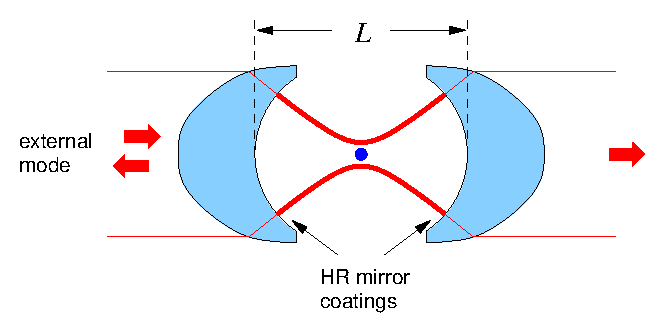
\includegraphics[width=\columnwidth]{cavitything.eps}

            \larger[2.5]

 	$ {\mathrm{C}= \frac{\mathrm{g_0}^{2}}{2\kappa\mathrm{\gamma}}}
            $   
       
    \columnbreak


            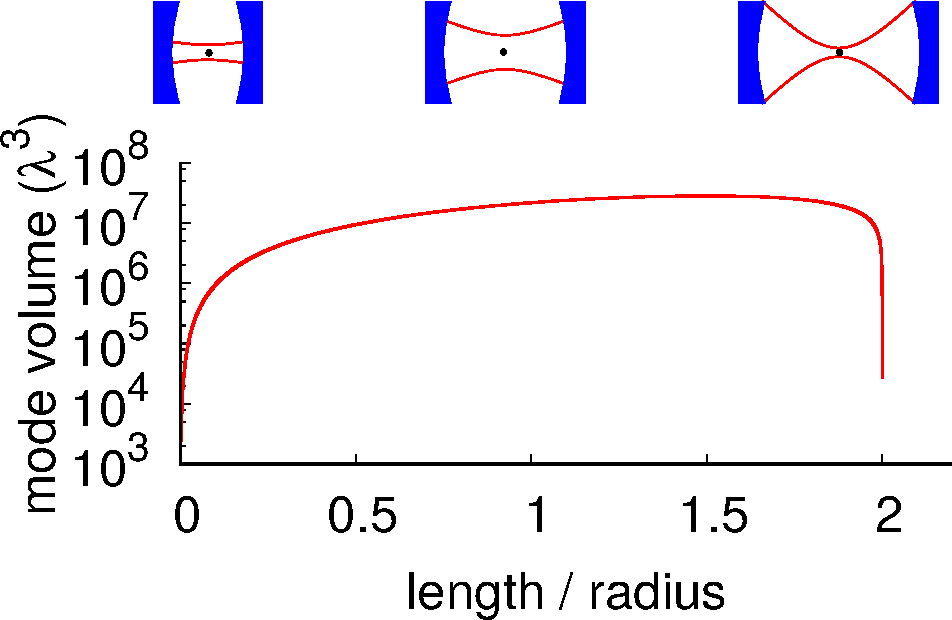
\includegraphics[width=\columnwidth]{mode_vol.pdf}

        \end{center}
	\end{multicols}


\vspace{-1cm}

  \figcaption{(Left) A nearly concentric cavity with a strongly focused mode. (Right) The calculated effective mode volume versus length of the cavity.}

\end{figurehere}

\begin{center}
  {\bf \Large \textsf {Cavity Construction}}
\end{center}

Near to the concentric point, which is at the edge of the stability regime,
the mode of the cavity is strongly focused and very sensitive
to alignment in all three directions. To be able to couple light in and out the cavity mode,
we employ an anaclastic lens-mirror design mounted on a three-axis PZT actuators. 

\begin{figurehere}
 
  \begin{center}
    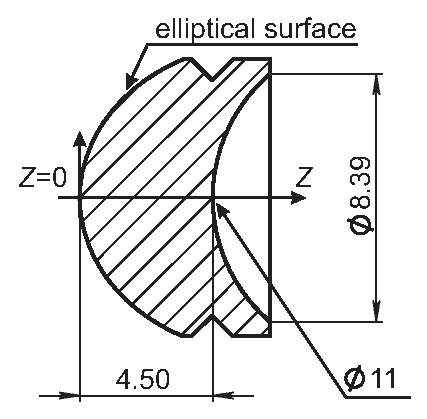
\includegraphics[height=8cm]{cavity_design}
   \hspace*{5cm}
    \includegraphics[height=8cm]{setup_sideon.png}
  \end{center}

\vspace{-1cm}

  \figcaption{(Left) Anaclastic lens-mirror design [2]. (Right) The movement of cavity mirrors  are controlled by a 3-axis PZT. }
\end{figurehere}



\begin{center}
     \begin{center} {\bf \Large \textsf {Experimental Setup}}\end{center}
\end{center}
The cavity used in the experiment has a finesse of 150 and a length of 4 $ \mathrm{\mu m}$ away from the concentric point. One of the longitudinal TEM$_{00}$ modes has a waist of 5 $ \mathrm{\mu m}$ and is near resonant with the $5^2 S_{1/2}$ F=2 $\rightarrow$ $5^2 P_{3/2}$ F'=3 transition of $^{87}$Rb at $\lambda=$ 780 nm. A second TEM$_{00}$ mode of the cavity, red detuned with respect to the first cavity mode is excited by a FORT trap laser at 810 nm, which is also used to continuously stabilize the cavity length. The laser cooled $^{87}$Rb atoms are loaded directly from a magneto optical trap (MOT) formed at the center of the cavity. The standing wave intracavity FORT with 1 mK trap depth captures and traps the MOT atoms at the antinode of the cavity mode. 
\begin{figurehere}
  \begin{center}
    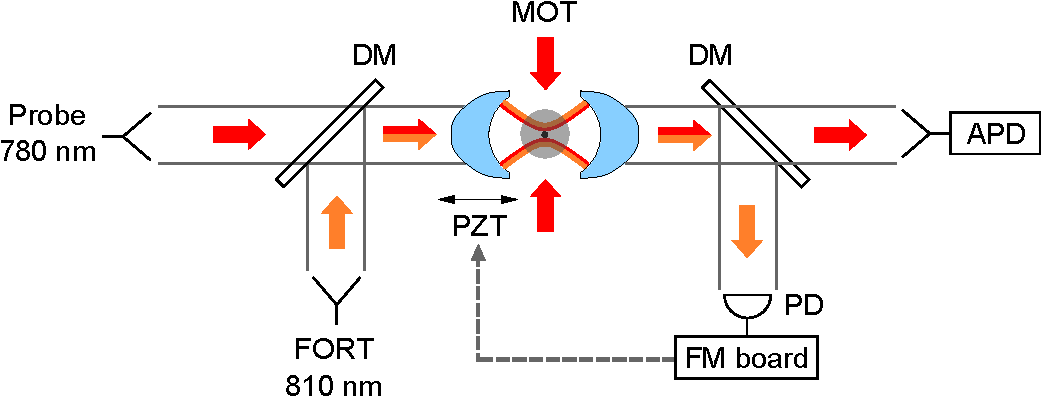
\includegraphics[width=0.8\columnwidth]{stabilise.pdf}
  \end{center}

\vspace{-1cm}

  \figcaption{Experimental setup. A single atom is trapped at the center of a nearly concentric cavity by way of an intracavity FORT at 810 nm. Probe and FORT beams with linear polarization are combined using a dichoric mirror (DM) and coupled to the same spatial TEM$_{00}$ mode of the cavity, where the output light of the FORT is used to stabilise the cavity length while the cavity transmission at 780 nm is coupled to a single mode fiber and detected by an APD.% and used to detect fluorescence signal from atoms as well as spectral response of the atom-cavity system.%   
  }
%%%%%%%%%%%%%%%%%%%%%
 % \figcaption{Experimental setup. A single atom is trapped at the center of the cavity by way of an intracavity FORT at 810nm. Probe and FORT beams are combined using a dichoric mirror (DM) and coupled to the same spatical TEM$_{00}$ mode of the cavity, where the transmission is then separated again using another DM. We use the output light from the FORT to stabilise the cavity length via frequency modulation (FM) technique. The cavity tranmission at 780nm is detected by an APD.   }
%%%%%%%%%%%%%%%%%%%%%

\end{figurehere}


\begin{center}
     \begin{center} {\bf \Large \textsf {Fluorescence Signal}}\end{center}
\end{center}
To determine if single atoms are loaded, we monitor the atomic fluorescence into cavity mode. Above a set threshold, the fluorescence signal triggers the experiment to begin.


\begin{figurehere}
  \begin{center}
    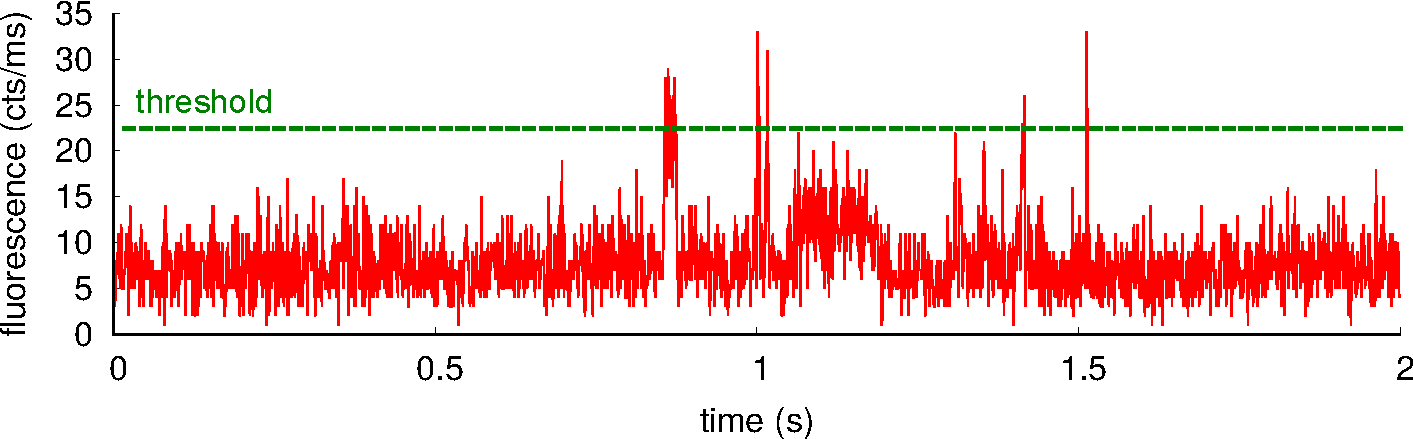
\includegraphics[width=0.8\columnwidth]{fluo_signal.pdf}
  \end{center}

\vspace{-1cm}

  \figcaption{ Time trace of fluorescence signal of the trapped atoms detected by APD. The sudden increase of the fluorescence signify the successful atom loading. }

\end{figurehere}

\columnbreak

After each successful triggering events, we interrupted the loading process by switching off the trapping magnetic field and analyze the fluorescence signal to determine whether a single atom is trapped. We estimate the probability of a successful loading of single atoms into our trap is around 30\%. 

\begin{figurehere}
  \begin{center}
    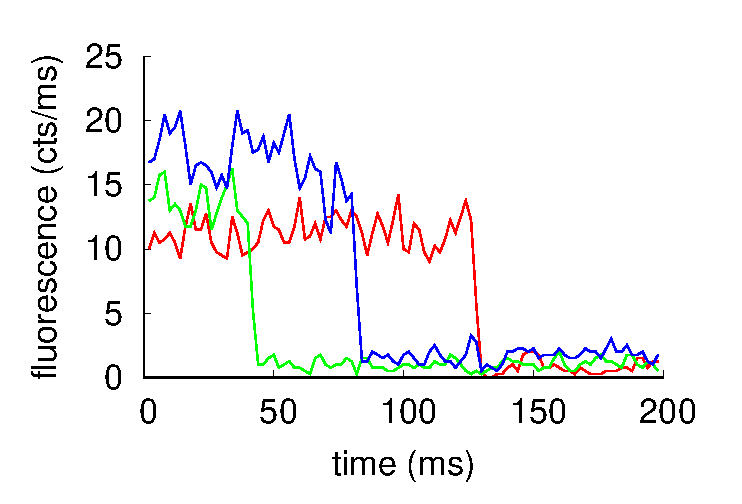
\includegraphics[width=0.48\columnwidth]{Plots/SA.eps}
   \hspace*{0cm}
    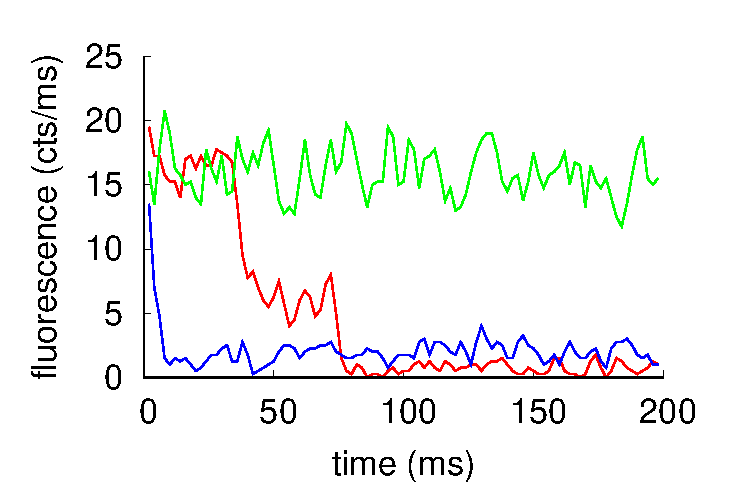
\includegraphics[width=0.48\columnwidth]{Plots/NSA.eps}
  \end{center}

\vspace{-1cm}

\figcaption{Samples of fluorescence signals due to a trapped single atom (left), a few atoms or inconclusive cases (right).}
\end{figurehere}



\begin{center}
  {\bf \Large \textsf {Transmission Signal}}
\end{center}

To study the interaction between the cavity and single atoms, we send alternating 1 ms pulses of weak probe laser and MOT laser and monitor the transmission and fluorescence of the cavity. The interleaving pulses and the dual-monitoring method allows us to post-select the single atom events and to determine when the trapped atom escapes out from the cavity mode. 

\begin{figurehere}
  \begin{center}
    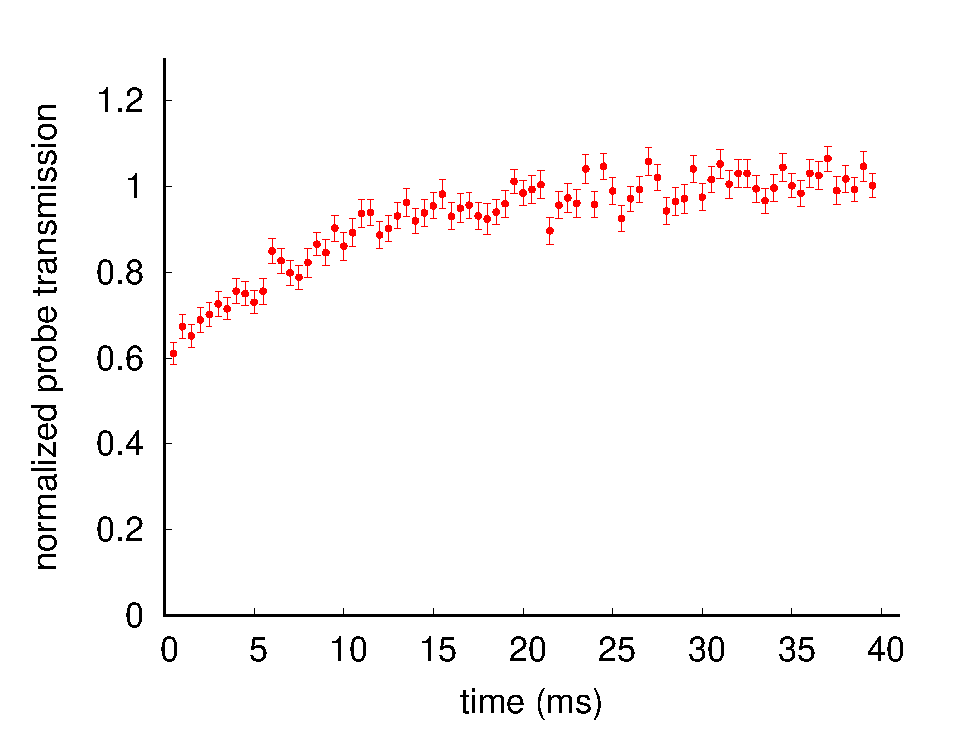
\includegraphics[width=0.6\columnwidth]{extinction_norm.eps}
  \end{center}

\vspace{-2cm}

    \figcaption{Average of transmission signal for all triggering events. The probe frequency is tuned to atom-cavity resonance to observe high extinction. The transmission signal recovers as the single atom escapes out of the cavity mode.}
\end{figurehere}



\begin{center}
  {\bf \Large \textsf {Normal Mode Splitting}}
\end{center}

We observed normal mode splitting in the cavity transmission spectrum due to the presence of a single atom in the cavity mode. The CQED system parameters are estimated to be $(g,\kappa,\gamma) = 2 \pi \times (10,40,3) \, \mathrm{MHz} $, with the single atom cooperativity $C=0.4$ putting our system into the intermediate coupling regime.

\begin{figurehere}
  \begin{center}
    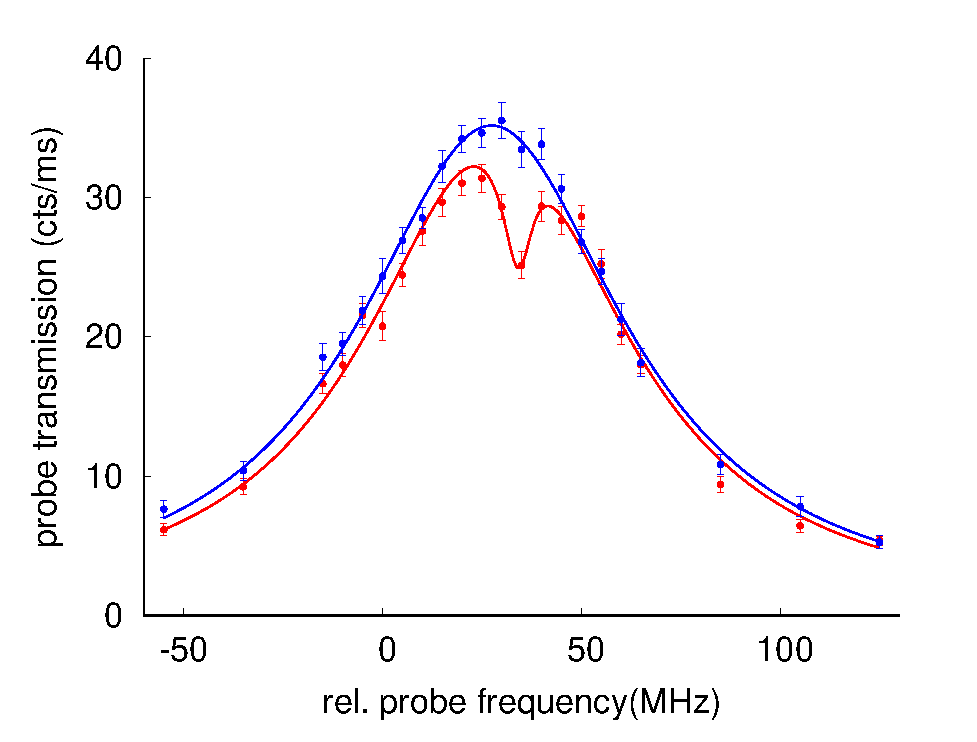
\includegraphics[width=0.6\columnwidth]{Plots/nsplit.eps}
  \end{center}

\vspace{-1cm}

    \figcaption{Cavity transmission spectrum of a weak probe laser, with no trapped atoms (blue) and a trapped single atom (red). The cavity is tuned close ($\sim 5 \, \mathrm{MHz}$) to the atomic resonance (shifted $34 \pm 2 \, \mathrm{MHz}$ from bare resonance due to a.c. stark shift from the FORT laser). The solid lines represent best fit to Lorentzian model (blue) and semiclassical CQED model (red).
}
\end{figurehere}


\begin{center}
  {\bf \Large \textsf {Outlook}}
\end{center}

We demonstrate an operational intermediate coupling CQED system in nearly concentric regime with huge physical volume and relatively low finesse cavity. We hope to move towards strong coupling regime in the near future by replacing the cavity mirrors with the ones with higher finesse. Successful realisation of such CQED system will open opportunities for further explorations in strong atom-photon interaction and increase the scalability for applications in quantum computing. 
\begin{flushleft}
       \begin{center}{\bf \large \textsf {References}}\end{center}
       [1] M.K. Tey et.al., New Journal of Physics {\textbf{11}}, 040311 (2009).
	     \newline
       %[2] S.E. Morin, et al., Phys.Rev.Lett., {\textbf {73}} pp.1411 (1994).
       %\newline
	     [2] K. Durak et.al., New Journal of Physics {\textbf{16}}, 103002 (2014).

\end{flushleft}

\end{multicols}

\end{poster}

\end{document}
